% -*- coding: UTF-8 -*-
% vim: autoindent expandtab tabstop=4 sw=4 sts=4 filetype=tex
% vim: spelllang=de spell
% chktex-file 27 - disable warning about missing include files

\chapter{Software-Architektur}
\label{chap:software-architecture}

\todo[inline]{Describe software architecture.}

Als Grundlage zur Entwicklung der Software-Architektur
dient~\citetitle{larman_applying_2004} von~\citeauthor{larman_applying_2004}.

Da~\cite{larman_applying_2004} auf dem Unified Process
(UP)~\cite{jacobson_unified_1999} basiert, wird vor allem dieser angewendet.
Dies hat ein iteratives Arbeiten zur Folge, da sich der UP auf agile Ansätze
wie Extreme Programming (XP) und Scrum fokussiert.

\todo[inline]{Describe general process}.
Process overview:
\begin{itemize}
    \item{Requirements}
    \item{Use cases}
    \item{Domain Models}
    \item{System Sequence Diagrams}
    \item{Packages}
    \item{Sequence Diagrams}
    \item{Class Diagrams}
    \item{Activity Diagrams}



% Sofern im Text nicht anders vermerkt, basiert das folgende Kapitel
% auf~\cite[S. 721ff]{foley_computer_1996}.
% 
% Für die Erzeugung und Darstellung von Bildern werden zwei Angaben
% benötigt: Was dargestellt werden soll und wie dieses dargestellt werden
% soll.
% Prinzipiell geht es darum zu bestimmen, welche Farbe eine Oberfläche an
% einem bestimmten Punkt hat. Dabei haben sich die Begriffe des
% \textit{Beleuchtungsmodelles (illumination model)} und des
% \textit{Modelles zur Schattierung (shading model)} etabliert.
% 
% \citeauthor{foley_computer_1996} nutzt den Begriff \textit{shading
% model} als Überbegriff~\parencite[S. 721]{foley_computer_1996}. Dieser
% schliesst auch Beleuchtungsmodelle ein.  Ein \textit{shading model}
% definiert, wann und mit welchen Parametern ein Beleuchtungsmodell
% angewendet wird. So nutzen manche \textit{shading models} ein
% Beleuchtungsmodell für jeden Pixel, andere wiederum nur für einzelne
% Pixel und interpolieren dabei die Werte der anderen Pixel.

% \input{inc/50/51_illumination_models}
% \input{inc/50/52_shading}

% -*- coding: UTF-8 -*-
% vim: autoindent expandtab tabstop=4 sw=4 sts=4 filetype=tex
% vim: spelllang=de spell
% chktex-file 27 - disable warning about missing include files

\section{Anforderungen}
\label{sec:requirements}

\subsection{Vision}
\label{subsec::requirements:vision}

Der Autor dieser Projektarbeit stellt sich eine Software zur Verwaltung und
Darstellung von Echtzeit-Animationen vor. Die Software soll es Anwendern erlauben
Echtzeit-Animationen in intuitiver Weise zu erstellen. Sie soll zudem modular
gehalten sein, so dass spätere Änderungen, wie z.B.\ zusätzliche Arten von
Rendering, ohne Weiteres adaptierbar sind.

\todo[inline]{Insert GUI mock-up here}

\subsection{Hauptkomponenten}
\label{subsec::requirements:main-components}

Die Applikation besteht aus zwei Applikationen: Einem \textit{Player},
welcher dem Abspielen von Echtzeit-Animationen dient, sowie einem \textit{Editor},
welcher der Erstellung und Verwaltung von Echtzeit-Animationen dient.

Der \textit{Editor} erlaubt den Export von erstellten Animationen inklusive den
dazugehörigen Dateien, wie zum Beispiel Bitmaps oder Modellen. Der
\textit{Player} kann die exportierten Animationen dann lesen und wiedergeben.

\subsection{Akteure (actors)}
\label{subsec::requirements:actors}

\textit{Primäre Akteure}
\begin{itemize}
    \item{%
            \textbf{Anwender}\\
            Ein \textit{Anwender} erstellt Echtzeit-Animationen mit der
            Software. Er hat also eine aktive Rolle.
        }
    \item{%
            \textbf{Betrachter}\\
            Ein \textit{Betrachter} nutzt die Software um eine durch den
            \textit{Anwender} erstellte Echtzeit-Animation anzusehen. Er nimmt
            also eine passive Rolle ein.
        }
\end{itemize}
\textit{Sekundäre Akteure}
\begin{itemize}
    \item{%
            \textbf{Entwickler}\\
            Ein \textit{Entwickler} erweitert die Software um neue Elemente
            (wie z.B.\ neue Shader).
        }
\end{itemize}

% -*- coding: UTF-8 -*-
% vim: autoindent expandtab tabstop=4 sw=4 sts=4 filetype=tex
% vim: spelllang=de spell
% chktex-file 27 - disable warning about missing include files

\subsection{Use Cases}
\label{subsec::requirements:use-cases}

Bei Use Cases handelt es sich um Anforderungen, genauer gesagt um funktionelle
bzw. Anforderungen an das Verhalten eines Systems~\cite{larman_applying_2004}.
Sie sagen also aus, was ein System tut bzw.\ tun soll. Die nachfolgenden Use
Cases sind keinesfalls vollständig --- dann wäre der Sinn des UP bzw.\ eines
iterativen Vorgehens verfehlt. Sie entwickeln sich viel mehr über die Zeit mit
dem Fortschreiten der Umsetzung.

% -*- coding: UTF-8 -*-
% vim: autoindent expandtab tabstop=4 sw=4 sts=4 filetype=tex
% vim: spelllang=de spell
% chktex-file 27 - disable warning about missing include files

\begin{table}[H]
    \centering
    \caption{Use Case UC1: Betrachten einer Echtzeit-Animation.}\label{table:uc1-watch-demo}
    \begin{tabular}{p{0.5\textwidth}p{0.5\textwidth}}
        \toprule
            \textbf{Bereich} &
            Player\\
        \cmidrule(r){1-1}\cmidrule(lr){2-2}
            \textbf{Level} &
            Ziel des Benutzers \\
        \cmidrule(r){1-1}\cmidrule(lr){2-2}
            \textbf{Primärer Aktor} &
            Betrachter \\
        \cmidrule(r){1-1}\cmidrule(lr){2-2}
            \textbf{Stakeholder und Interessen} &
            Betrachter: Möchte eine zuvor erstellte Echtzeit-Animation ansehen.  \newline
            Anwender: Testen einer erstellen Echtzeit-Animation. \newline
            Entwickler: Testen einer erstellen Echtzeit-Animation. \\
        \cmidrule(r){1-1}\cmidrule(lr){2-2}
            \textbf{Erfolgsszenario} &
            \begin{enumerate}
                \item{Der Betrachter startet die Player-Applikation und wählt
                        die gewünschten Optionen, wie Auflösung und Bit-Tiefe.}
                \item{Der Betrachter startet die Animation.}
                \item{Der Player spielt die Animation bis zum Ende.}
                \item{Der Player wird automatisch geschlossen.}
            \end{enumerate} \\
        \cmidrule(r){1-1}\cmidrule(lr){2-2}
            \textbf{Erweiterungen} &
            \begin{enumerate}[label= (\alph*)]
                \item{Vorzeitiger Abbruch durch den Betrachter
                    \begin{enumerate}[label= (\roman*)]
                            \item{Der Betrachter bricht eine laufende Animation
                                    ab.}
                            \item{Der Player wird sofort geschlossen.}
                    \end{enumerate}
                }
                \item{Absturz/Ausfall des Systems
                    \begin{enumerate}[label= (\roman*)]
                            \item{Das System stürzt an einem beliebigen Punkt
                                    ab.}
                            \item{Neustart des Players.}
                            \item{Der Player beginnt die Animation von vorne.}
                    \end{enumerate}
                }
            \end{enumerate}
            \\
        \cmidrule(r){1-1}\cmidrule(lr){2-2}
            \textbf{Zusätzliche Anforderungen} &
            \todo[inline]{Add add. requirements} \\
        \bottomrule
    \end{tabular}
\end{table}


% -*- coding: UTF-8 -*-
% vim: autoindent expandtab tabstop=4 sw=4 sts=4 filetype=tex
% vim: spelllang=de spell
% chktex-file 27 - disable warning about missing include files

\subsubsection{Use Case UC2: Erstellen einer Echtzeit-Animation}
\label{ssubsec:requirements:use-cases:uc2}

\begin{longtabu}{p{0.5\textwidth}p{0.5\textwidth}}
    \centering\\
    \caption{Use Case UC2: Erstellen einer
        Echtzeit-Animation.}\label{table:uc2-create-demo}\\
    \toprule
        \textbf{Bereich} &
        Editor \\
    \cmidrule(r){1-1}\cmidrule(lr){2-2}
        \textbf{Stufe (level)} &
        Ziel des Benutzers \\
    \cmidrule(r){1-1}\cmidrule(lr){2-2}
        \textbf{Primärer Aktor} &
        Anwender \\
    \cmidrule(r){1-1}\cmidrule(lr){2-2}
        \textbf{Stakeholder und Interessen} &
        Anwender: Möchte eine neue Echtzeit-Animation erstellen.\newline
        Betrachter: Möchte eine erstellte Echtzeit-Animation ansehen. \\
    \cmidrule(r){1-1}\cmidrule(lr){2-2}
        \textbf{Vorbedingungen} &
        Der Editor sichert eine Animation alle \textit{n}-Minuten in einer
        temporären Sicherungsdatei. \\
    \cmidrule(r){1-1}\cmidrule(lr){2-2}
        \textbf{Erfolgsszenario} &
        \begin{enumerate}
            \item{Der Anwender startet die Editor-Applikation.}
            \item{Der Anwender fügt Elemente zu einer Szene zusammen.}
            \item{Der Anwender legt Start und Ende einer Animation fest.}
            \item{Der Anwender speichert die getätigte Arbeit.}
            \item{Der Anwender exportiert die erstellte Animation.}
            \item{Der Anwender schliesst den Editor.}
        \end{enumerate} \\
    \cmidrule(r){1-1}\cmidrule(lr){2-2}
        \textbf{Erweiterungen} &
        \begin{enumerate}[label= (\alph*)]
            \item{Schliessen des Editors bei gemachten Änderungen ohne zu
                    speichern
                \begin{enumerate}[label= (\roman*)]
                    \item{Der Anwender schliesst den Editor bei gemachten
                            Änderungen ohne diese zu speichern.}
                    \item{Der Editor weist den Anwender auf die
                            nicht gespeicherten Änderungen hin und bietet
                            die Möglichkeit diese zu speichern, diese nicht
                            zu speichern oder das Schliessen abzubrechen.}
                \end{enumerate}
            }\\
        \end{enumerate}\\
    \cmidrule(r){1-1}\cmidrule(lr){2-2}
        \textbf{Fehlerfall} &
        \begin{enumerate}[label= (\alph*)]
            \item{Absturz/Ausfall des Systems
                \begin{enumerate}[label= (\roman*)]
                        \item{Das System stürzt an einem beliebigen Punkt
                                ab.}
                        \item{Neustart des Editors.}
                        \item{Der Editor stellt den ihm zuletzt bekannten
                                Punkt der Animation wieder her.}
                \end{enumerate}
            }
            \item{Es sind keine Elemente zum Hinzufügen vorhanden
                \begin{enumerate}[label= (\roman*)]
                    \item{Das Fenster zum Hinzufügen von Elementen ist leer.}
                \end{enumerate}
            }
            \item{Die getätigte Arbeit kann nicht gespeichert werden
                \begin{enumerate}[label= (\roman*)]
                    \item{Beim Speichern tritt ein Fehler auf.}
                    \item{Der Anwender wird via Dialog-Fenster über den Fehler
                            informiert.}
                    \item{Die Datei wird nicht gespeichert.}
                    \item{Die Datei gilt nach wie vor als geändert.}
                    \item{Die Datei muss zu einem späteren Zeitpunkt
                            gespeichert werden.}
                \end{enumerate}
            }
            \item{Die erstellte Animation kann nicht exportiert werden
                \begin{enumerate}[label= (\roman*)]
                    \item{Beim Exportieren tritt ein Fehler auf.}
                    \item{Der Anwender wird via Dialog-Fenster über den Fehler
                            informiert.}
                    \item{Die Datei wird nicht exportiert.}
                    \item{Die Datei muss zu einem späteren Zeitpunkt
                            exportiert werden.}
                \end{enumerate}
            }
        \end{enumerate} \\
    \cmidrule(r){1-1}\cmidrule(lr){2-2}
        \textbf{Zusätzliche Anforderungen} &
        Betreffend dem Exportieren ist das zu verwendende Format zum jetzigen
        Zeitpunkt noch unklar. In Frage käme zum Beispiel
        JSON\protect\footnotemark{} oder X3D\protect\footnotemark{}.\\
        \footnotetext{http://www.json.org/}
        \footnotetext{http://www.web3d.org/x3d}
    \bottomrule
\end{longtabu}

% -*- coding: UTF-8 -*-
% vim: autoindent expandtab tabstop=4 sw=4 sts=4 filetype=tex
% vim: spelllang=de spell
% chktex-file 27 - disable warning about missing include files

\begin{table}[H]
    \centering
    \caption{Use Case UC3: Bearbeiten einer bestehenden Animation}\label{table:uc3-edit-demo}
    \begin{tabular}{p{0.5\textwidth}p{0.5\textwidth}}
        \toprule
            \textbf{Bereich} &
            Editor \\
        \cmidrule(r){1-1}\cmidrule(lr){2-2}
            \textbf{Level} &
            Ziel des Benutzers \\
        \cmidrule(r){1-1}\cmidrule(lr){2-2}
            \textbf{Primärer Aktor} &
            Anwender \\
        \cmidrule(r){1-1}\cmidrule(lr){2-2}
            \textbf{Stakeholder und Interessen} &
            Anwender: Möchte eine zuvor erstellte Echtzeit-Animation verändern. \newline
            Betrachter: Möchte eine geänderte Echtzeit-Animation ansehen. \newline
            Entwickler: Testen einer geänderten Echtzeit-Animation. \\
        \cmidrule(r){1-1}\cmidrule(lr){2-2}
            \textbf{Erfolgsszenario} &
            \begin{enumerate}
                \item{Der Anwender startet die Editor-Applikation.}
                    \item{Der Anwender öffnet eine zuvor gespeicherte
                            Echtzeit-Animation.}
                \item{Der Editor lädt die gewählte Echtzeit-Animation.}
                \item{Der Anwender nimmt eine oder mehrere Änderungen vor.}
                \item{Der Anwender speichert die getätigte Arbeit.}
                \item{Der Anwender exportiert die erstellte Animation.}
                \item{Der Anwender schliesst den Editor.}
            \end{enumerate} \\
        \cmidrule(r){1-1}\cmidrule(lr){2-2}
            \textbf{Erweiterungen} &
            \begin{enumerate}[label= (\alph*)]
                \item{Schliessen des Editors bei gemachten Änderungen ohne zu
                        speichern
                    \begin{enumerate}[label= (\roman*)]
                        \item{Der Anwender schliesst den Editor bei gemachten
                                Änderungen ohne diese zu speichern.}
                        \item{Der Editor weist den Anwender auf die
                                nicht gespeicherten Änderungen hin und bietet
                                die Möglichkeit diese zu speichern, diese nicht
                                zu speichern oder das Schliessen abzubrechen.}
                    \end{enumerate}
                }
                \item{Eine zuvor gespeicherte Echtzeit-Animation kann nicht
                        geladen werden.
                    \begin{enumerate}[label= (\roman*)]
                        \item{Der Anwender öffnet eine zuvor gespeicherte
                                Echtzeit-Animation.}
                        \item{Der Editor weist den Anwender auf den Umstand
                                hin, dass die Echtzeit-Animation nicht geöffnet
                                werden kann.}
                    \end{enumerate}
                }
                \item{Benötigte zusätzliche Dateien können nicht gefunden
                        werden.
                    \begin{enumerate}[label= (\roman*)]
                        \item{Der Anwender öffnet eine zuvor gespeicherte
                                Echtzeit-Animation bei welcher benötigte
                                Dateien (wie zum Beispiel Bitmaps) fehlen.}
                        \item{Der Editor weist den Anwender auf den Umstand
                                hin, öffnet die Echtzeit-Animation dennoch. Er
                                ersetzt die fehlenden Dateien mit
                                Platzhaltern. Ein fehlerfreier Ablauf der
                                Echtzeit-Animation ist nicht gewährleistet.}
                    \end{enumerate}
                }
                \item{Absturz/Ausfall des Systems
                    \begin{enumerate}[label= (\roman*)]
                            \item{Das System stürzt an einem beliebigen Punkt
                                    ab.}
                            \item{Neustart des Editors.}
                            \item{Der Editor stellt den ihm zuletzt bekannten
                                    Punkt der Animation wieder her.}
                    \end{enumerate}
                }
            \end{enumerate}
            \\
        \cmidrule(r){1-1}\cmidrule(lr){2-2}
            \textbf{Zusätzliche Anforderungen} &
            \todo[inline]{Add add. requirements} \\
        \bottomrule
    \end{tabular}
\end{table}

% -*- coding: UTF-8 -*-
% vim: autoindent expandtab tabstop=4 sw=4 sts=4 filetype=tex
% vim: spelllang=de spell
% chktex-file 27 - disable warning about missing include files

\begin{table}[H]
    \centering
    \caption{Use Case UC4: Exportieren einer Animation.}\label{table:uc4-export-demo}
    \begin{tabular}{p{0.5\textwidth}p{0.5\textwidth}}
        \toprule
            \textbf{Bereich} &
            Editor \\
        \cmidrule(r){1-1}\cmidrule(lr){2-2}
            \textbf{Level} &
            Ziel des Benutzers \\
        \cmidrule(r){1-1}\cmidrule(lr){2-2}
            \textbf{Primärer Aktor} &
            Anwender \\
        \cmidrule(r){1-1}\cmidrule(lr){2-2}
            \textbf{Stakeholder und Interessen} &
            Anwender: Möchte eine erstellte Echtzeit-Animation für die
            Verwendung im Player exportieren. \newline
            Betrachter: Möchte eine Echtzeit-Animation ansehen. \newline
            Entwickler: Testen einer Echtzeit-Animation im Player. \\
        \cmidrule(r){1-1}\cmidrule(lr){2-2}
            \textbf{Erfolgsszenario} &
            \begin{enumerate}
                \item{Der Anwender startet die Editor-Applikation.}
                    \item{Der Anwender öffnet eine zuvor gespeicherte
                            Echtzeit-Animation oder erstellt eine neue
                            Echtzeit-Animation.}
                \item{Der Anwender speichert die getätigte Arbeit.}
                \item{Der Anwender exportiert die erstellte Animation.}
                \item{Der Editor exportiert die erstellte Animation mit allen
                        benötigen Abhängigkeiten in ein definiertes (Unter-)
                        Verzeichnis.}
                \item{Der Anwender schliesst den Editor.}
            \end{enumerate} \\
        \cmidrule(r){1-1}\cmidrule(lr){2-2}
            \textbf{Erweiterungen} &
            \begin{enumerate}[label= (\alph*)]
                \item{Schliessen des Editors bei gemachten Änderungen ohne zu
                        speichern
                    \begin{enumerate}[label= (\roman*)]
                        \item{Der Anwender schliesst den Editor bei gemachten
                                Änderungen ohne diese zu speichern.}
                        \item{Der Editor weist den Anwender auf die
                                nicht gespeicherten Änderungen hin und bietet
                                die Möglichkeit diese zu speichern, diese nicht
                                zu speichern oder das Schliessen abzubrechen.}
                    \end{enumerate}
                }
                \item{Eine zuvor gespeicherte Echtzeit-Animation kann nicht
                        geladen werden.
                    \begin{enumerate}[label= (\roman*)]
                        \item{Der Anwender öffnet eine zuvor gespeicherte
                                Echtzeit-Animation.}
                        \item{Der Editor weist den Anwender auf den Umstand
                                hin, dass die Echtzeit-Animation nicht geöffnet
                                werden kann.}
                    \end{enumerate}
                }
                \item{Benötigte zusätzliche Dateien können nicht gefunden
                        werden.
                    \begin{enumerate}[label= (\roman*)]
                        \item{Der Anwender öffnet eine zuvor gespeicherte bzw.
                                erstellt eine neue Echtzeit-Animation bei
                                welcher benötigte Dateien (wie zum Beispiel
                                Bitmaps) fehlen.}
                        \item{Der Editor weist den Anwender auf den Umstand
                                hin, exportiert die Echtzeit-Animation dennoch. Er
                                ersetzt die fehlenden Dateien mit
                                Platzhaltern. Ein fehlerfreier Ablauf der
                                Echtzeit-Animation ist nicht gewährleistet.}
                    \end{enumerate}
                }
                \item{Absturz/Ausfall des Systems
                    \begin{enumerate}[label= (\roman*)]
                            \item{Das System stürzt an einem beliebigen Punkt
                                    ab.}
                            \item{Neustart des Editors.}
                            \item{Der Editor stellt den ihm zuletzt bekannten
                                    Punkt der Animation wieder her.}
                    \end{enumerate}
                }
            \end{enumerate}
            \\
        \cmidrule(r){1-1}\cmidrule(lr){2-2}
            \textbf{Zusätzliche Anforderungen} &
            \todo[inline]{Add add. requirements} \\
        \bottomrule
    \end{tabular}
\end{table}

% -*- coding: UTF-8 -*-
% vim: autoindent expandtab tabstop=4 sw=4 sts=4 filetype=tex
% vim: spelllang=de spell
% chktex-file 27 - disable warning about missing include files

\begin{table}[H]
    \centering
    \caption{Use Case UC5: Bereitstellen neuer Editor-Elemente.}\label{table:uc1-user}
    \begin{tabular}{p{0.5\textwidth}p{0.5\textwidth}}
        \toprule
            \textbf{Bereich} &
            Player\\
        \cmidrule(r){1-1}\cmidrule(lr){2-2}
            \textbf{Level} &
            Ziel des Benutzers \\
        \cmidrule(r){1-1}\cmidrule(lr){2-2}
            \textbf{Primärer Aktor} &
            Entwickler \\
        \cmidrule(r){1-1}\cmidrule(lr){2-2}
            \textbf{Stakeholder und Interessen} &
            Entwickler: Möchte dem Anwender neue Möglichkeiten zur visuellen
            Gestaltung bieten. Möchte dem Betrachter neue, visuell ansprechende
            Elemente bieten. \newline
            Anwender: Möchte neue Funktionen zur Erstellung von
            Echtzeit-Animation nutzen können. \newline
            Betrachter: Möchte visuell ansprechende Echtzeit-Animationen mit
            neuen Effekten ansehen. \\
        \cmidrule(r){1-1}\cmidrule(lr){2-2}
            \textbf{Erfolgsszenario} &
            \begin{enumerate}
                \item{Der Entwickler entwickelt neuen Inhalt in Form eines
                        Knotens für den Graphen (dies kann zum Beispiel ein
                        prozedurales Mesh oder ein dedizierter Shader sein).}
                \item{Der Entwickler startet den Editor.}
                \item{Der neue Knoten steht im Editor automatisch zur Verfügung
                        und kann genutzt werden.}
                \item{Der Entwickler schliesst den Editor.}
            \end{enumerate} \\
        \cmidrule(r){1-1}\cmidrule(lr){2-2}
            \textbf{Erweiterungen} &
            \begin{enumerate}[label= (\alph*)]
                \item{Erfassen neuer Knoten direkt im Editor
                    \begin{enumerate}[label= (\roman*)]
                        \item{Der Entwickler startet den Editor.}
                        \item{Der Entwickler öffnet die Bibliothek mit allen
                                Knoten-Typen.}
                        \item{Der Entwickler fügt der Bibliothek einen neuen
                                Knoten hinzu.}
                        \item{Der Entwickler füllt den Knoten mit den
                                entsprechenden Details und speichert diesen.}
                        \item{Der neu erstellte Knoten wird persistiert.}
                        \item{Der neu erstellte Knoten erscheint in der
                                Bibliothek und ist per sofort auswählbar.}
                        \item{Der Entwickler schliesst den Editor.}
                    \end{enumerate}
                }
                \item{Fehlerhafter Inhalt des Knotens
                    \begin{enumerate}[label= (\roman*)]
                        \item{Der Entwickler fügt dem Knoten keinen oder
                                fehlerhaften Inhalt hinzu.}
                        \item{Der Editor weist den Entwickler auf den Umstand
                                hin. Der Knoten kann nicht verwendet werden.}
                    \end{enumerate}
                }
                \item{Absturz/Ausfall des Systems
                    \begin{enumerate}[label= (\roman*)]
                            \item{Das System stürzt an einem beliebigen Punkt
                                    ab.}
                            \item{Neustart des Editors.}
                            \item{Der Editor stellt den ihm zuletzt bekannten
                                    Punkt der Animation wieder her.}
                    \end{enumerate}
                }
            \end{enumerate}
            \\
        \cmidrule(r){1-1}\cmidrule(lr){2-2}
            \textbf{Zusätzliche Anforderungen} &
            \todo[inline]{Add add. requirements} \\
        \bottomrule
    \end{tabular}
\end{table}



% -*- coding: UTF-8 -*-
% vim: autoindent expandtab tabstop=4 sw=4 sts=4 filetype=tex
% vim: spelllang=de spell
% chktex-file 27 - disable warning about missing include files

\subsection{Zusätzliche Anforderungen}
\label{subsec:requirements:additional-requirements}

\subsubsection{Software}
\label{subsec:requirements:additional-requirements:software}

Durch die vorhergehende Projektarbeit --- MTE7101
(siehe~\cite{osterwalder_sven_volume_2016}) --- sowie persönlicher Erfahrungen
bei diversen Projekten, sieht der Autor die Software gemäss
Tabelle~\ref{table:requirements:additional-requirements:software} zur Umsetzung
vor. Alle genannten Komponenten --- ausser Qt --- beziehen sich auf den
\textit{Player}, als auch auf den \textit{Editor}.  Der Player benötigt kein
Qt, da er kein Frontend hat und möglichst schlank gehalten werden soll.

% Sigh..
% FYI:  Tabular and a fixed text-width of 79 sucks!
% FYI2: set cursorcolumn with a lot of text sucks too!

\begin{longtabu}{p{0.2\textwidth}p{0.1\textwidth}p{0.6\textwidth}p{0.1\textwidth}}
    \caption{Mögliche
        Software/Technologien}\label{table:requirements:additional-requirements:software}\\
    \toprule
    \textbf{Komponente} & \textbf{Version} & \textbf{Beschreibung} & \textbf{Verweise} \\
    \midrule
    C++        & 11      & Objektorientierte Programmiersprache
                           & \protect\footnotemark\footnotetext{
                               \url{http://www.iso.org/iso/iso_catalogue/catalogue_tc/catalogue_detail.htm?csnumber=50372}
                           }\\

    OpenGL     & 4.5     & Plattformunabhängige Programmierschnittstelle zur
                           Entwicklung von 2D- und 3D-Computergrafikanwendungen
                           \parencite{wikipedia_the_free_encyclopedia_opengl_2015}
                           &\protect\footnotemark\footnotetext{
                               \url{https://www.opengl.org/registry/doc/glspec45.core.pdf}
                           }\\

    Qt        & 5.7      & ``Qt ist eine C++-Klassenbibliothek für die
                           plattformübergreifende Programmierung grafischer
                           Benutzeroberflächen. Außerdem bietet Qt
                           umfangreiche Funktionen zur Internationalisierung
                           sowie Datenbankfunktionen und XML-Unterstützung an
                           und ist für eine große Zahl an Betriebssystemen bzw.
                           Grafikplattformen, wie X11 (Unix-Derivate), OS X,
                           Windows, iOS und Android
                           erhältlich.''~\parencite{wikipedia_foundation_qt_2016}.
                           &\protect\footnotemark\footnotetext{
                               \url{https://www.qt.io}
                           }\\

    GLFW       & 3.1.2   & OpenGL-Bibliothek, welche die Erstellung und
                           Verwaltung von Fenstern sowie OpenGL-Kontexte
                           vereinfacht
                           \parencite{wikipedia_the_free_encyclopedia_glfw_2015}.
                           &\protect\footnotemark\footnotetext{
                               \url{http://www.glfw.org}
                           }\\

    GLEW       & 1.13    & OpenGL Extension Wrangler. Bibliothek zum Abfragen
                           und Laden von OpenGL-Erweiterungen (Extensions)
                           \parencite{wikipedia_the_free_encyclopedia_opengl_2015-1}.
                           &\protect\footnotemark\footnotetext{
                               \url{http://glew.sourceforge.net}
                           }\\

    GLM        & 0.9.7.6 & Header-only C++ Mathematik-Bibliothek, basierend auf
                           der Spezifikation der OpenGL Shader-Sprache GLSL.
                           Sie bietet eine Vielzahl an Datentypen wie etwa
                           Vektoren, Matrizen oder Quaternionen.
                           &\protect\footnotemark\footnotetext{
                               \url{https://glm.g-truc.net}
                           }\\

    CMake      & 3.3.2   & Software zur Verwaltung von Build-Prozessen von 
                           Software
                           &\protect\footnotemark\footnotetext{
                               \url{https://www.cmake.org}
                           }\\

    LLVM       & 3.8.1   & Ansammlung von modularen und wiederverwendbaren
                           Compilern und Toolchains.
                           &\protect\footnotemark\footnotetext{
                               \url{http://llvm.org}
                           }\\

    Clang      & 3.8.1   & Compiler-Frontend für LLVM.\@
                           &\protect\footnotemark\footnotetext{
                               \url{http://clang.llvm.org}
                           }\\

    Boost      & 1.59.0  & Freie Bibliothek bestehend aus einer Vielzahl von
                           Bibliotheken, die den unterschiedlichsten
                           Aufgaben von Algorithmen auf Graphen über 
                           Metaprogrammierung bis hin zu Speicherverwaltung
                           dienen
                           \parencite{wikipedia_the_free_encyclopedia_boost_2015}.
                           &\protect\footnotemark\footnotetext{
                               \url{http://www.boost.org}
                           }\\
    \bottomrule
\end{longtabu}


% -*- coding: UTF-8 -*-
% vim: autoindent expandtab tabstop=4 sw=4 sts=4 filetype=tex
% vim: spelllang=de spell
% chktex-file 27 - disable warning about missing include files

\section{Domänenmodell}
\label{sec:domain-model}

Der wesentliche Schritt der objektorientierten Analyse ist die Zerlegung einer
Domäne in essentielle Konzepte oder Objekte~\cite[S. 134]{larman_applying_2004}.

In UML wird ein Domänenmodell typischerweise als eine Menge von
Klassendiagrammen ohne Operationen dargestellt. Es liefert eine konzeptuelle
Perspektive und kann folgende Elemente beinhalten~\cite[S. 134]{larman_applying_2004}:
\begin{itemize}
    \item{Objekte der Domäne oder konzeptuelle Klassen}
    \item{Relationen zwischen konzeptuellen Klassen}
    \item{Attribute der konzeptuellen Klassen}
\end{itemize}

\citeauthor{larman_applying_2004} weist darauf hin, dass nicht versucht werden
sollte von Beginn weg ein möglichst genaues, vollständiges oder ``korrektes''
Domänenmodell zu erstellen. Ein solcher Ansatz führt zu ``analysis paralysis''
und sollte daher vermieden werden, da dies wenig bis keinen Mehrwert
bring~\cite[S. 133]{larman_applying_2004}.

Da angedacht ist, dass die Software aus zwei Applikationen, dem
\textit{Player} sowie dem \textit{Editor}, besteht, wird für jede
Applikation ein Domänenmodell erstellt.

\subsection{Player}
\label{subsec:domain-model:player}

\begin{figure}[H]
    \centering
    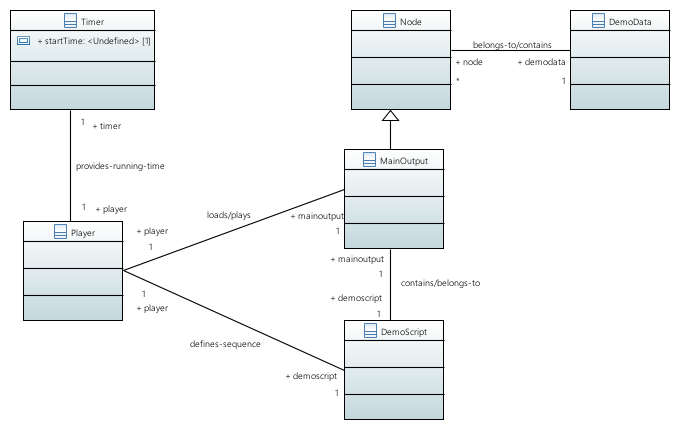
\includegraphics[width=0.8\textwidth]{img/player_domain_model.png}
    \caption{Domänenmodell der
        Player-Applikation\protect\footnotemark}\label{fig:domain-model:player}
\end{figure}
\footnotetext{Eigene Darstellung mittels Papyrus.}

Abbildung~\ref{fig:domain-model:player} zeigt das Domänenmodell der
Player-Applikation. Das Modell ist bewusst minimal gehalten und zeigt nur die
nötigsten Komponenten. Im Zentrum steht das Player-Objekt. Dieses liest ein
DemoScript, welches eine exportiert Echtzeit-Animation des Editors darstellt.
Ausgehend vom DemoScript kann schliesslich der Hauptknoten des Graphen gefunden
evaluiert werden. Ausgehend von diesem wird so die gesamte Echtzeit-Animation
aufgebaut und wiedergeben.

Viele essentielle Konzepte beziehungsweise Objekte fehlen in diesem Modell
bewusst. Diese werden während den Iterationen der darauffolgenden Projektarbeit
erarbeitet. Ein Teil davon findet sich im Domänenmodell des Editors
(\ref{subsec:domain-model:editor}) sowie im Klassendiagramm des Prototypen
(\ref{chap:prototype}).

\subsection{Editor}
\label{subsec:domain-model:editor}

\begin{figure}[H]
    \centering
    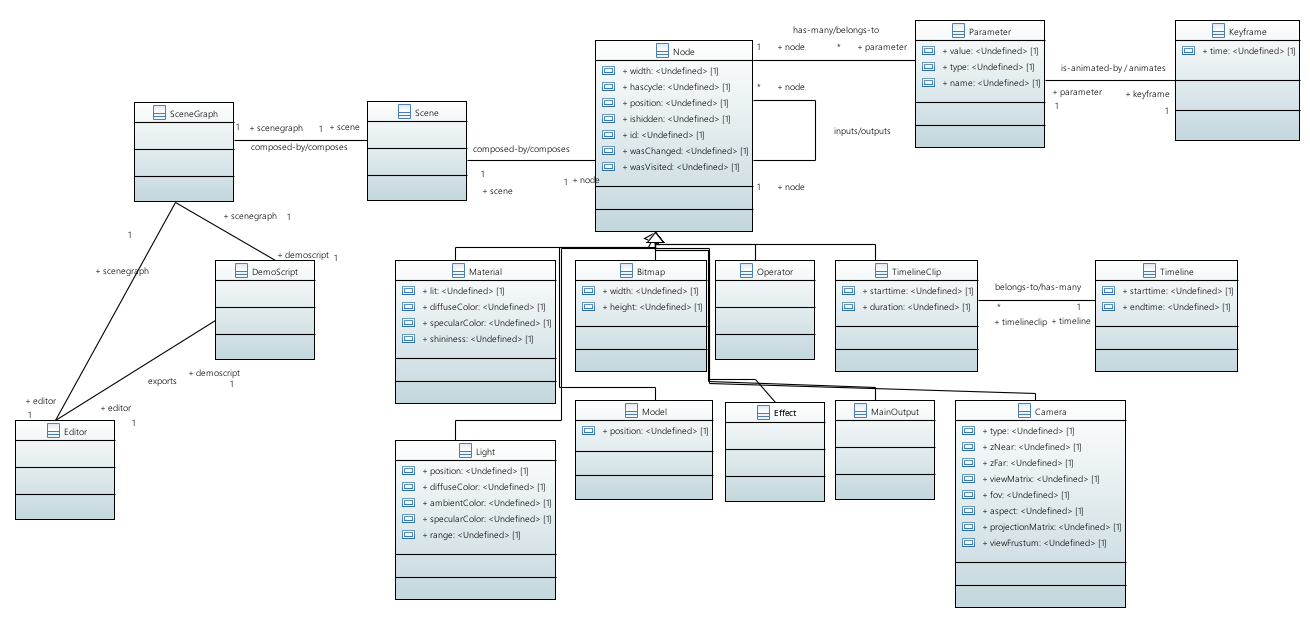
\includegraphics[angle=90,width=0.6\textwidth]{img/editor_domain_model.png}
    \caption{Domänenmodell der
        Editor-Applikation\protect\footnotemark}\label{fig:domain-model:editor}
\end{figure}
\footnotetext{Eigene Darstellung mittels Papyrus.}

Abbildung~\ref{fig:domain-model:editor} zeigt das Domänenmodell der
Editor-Applikation. Analog dem vorherigen Modell steht hier das Editor-Objekt
im Zentrum. Dieses bildet die Schnittstelle zwischen der grafischen
Benutzeroberfläche (GUI) und der Applikationslogik.

Die Komponenten der grafischen Benutzeroberfläche wurden in diesem Modell
bewusst weggelassen, da dies das Modell nur unnötig vergrössern würde. Die
eigentliche Logik findet sich in den essentiellen Konzepten beziehungsweise in
den hier gezeigten Objekten. Die grafische Benutzeroberfläche bildet diese nur
ab respektive Kopien davon.

Im mittleren Teil ist mit dem Node-Objekt und dessen Spezialisierung die
gesamte Struktur des Graphen angedeutet. Dies werden schliesslich die Objekte
sein, welche ein Anwender nutzen kann um Echtzeit-Animationen zu erstellen.

Im rechten Teil des Modelles stellen die Objekte Parameter, Keyframe,
TimelineClip und Timeline Elemente zur Animation dar. Pro Parameter kann zu
einem bestimmten Zeitpunkt der Zeitachse ein Schlüsselbild (Keyframe) gesetzt
werden. Timeline stellt die gesamte Zeitachse und TimelineClip einzelne
Elemente dieser dar. Es handelt sich bei Letzteren um Szenen.

Auch hier fehlen wiederum etliche Details, wie zum Beispiel das gesamte
Rendering inklusive den Shadern. Ein Teil davon ist wiederum im Klassendiagramm
des Prototypen (\ref{chap:prototype}) ersichtlich.

Wie Eingangs erwähnt, ist es nicht das Ziel ein vollständiges oder
``korrektes'' Domänenmodell zu erstellen. Es geht viel mehr um einen ersten
Anstoss zur eigentlichen Implementierung. Alle weiteren Details werden während
den Iterationen der darauffolgenden Projektarbeit erarbeitet.

% -*- coding: UTF-8 -*-
% vim: autoindent expandtab tabstop=4 sw=4 sts=4 filetype=tex
% vim: spelllang=de spell
% chktex-file 27 - disable warning about missing include files

\section{Sequenz-Diagramme}
\label{sec:sequence-diagrams}

Gemäss~\cite{larman_applying_2004} stellen Sequenz-Diagramme Ereignisse, welche
externe Akteure auslösen bzw.\ generieren, deren Ablauf sowie Ereignisse
zwischen Systemen eines spezifischen Szenarios eines Use Cases dar.

Da Sequenz-Diagramme schnell eine gewisse Grösse und auch Komplexität annehmen
wird in dieser Projektarbeit darauf verzichtet ein Sequenz-Diagramm für alle
Use Cases zu erstellen. Gerade bei \```UC2: Erstellen einer
Echtzeit-Animation\''' würde dies ansonsten grosse Ausmasse annehmen. Bei
Bedarf können diese bei den einzelnen Iterationen bzw.\ Phasen (Elaboration,
Construction und Transition). An dieser Stelle wird daher nur das
Sequenz-Diagramm für den ersten Use Case, \```UC1: Betrachten einer
Echtzeit-Animation\''' dargestellt. Dies deckt bereits einen Teil des Editors
mit ab.

\begin{figure}[H]
    \centering
    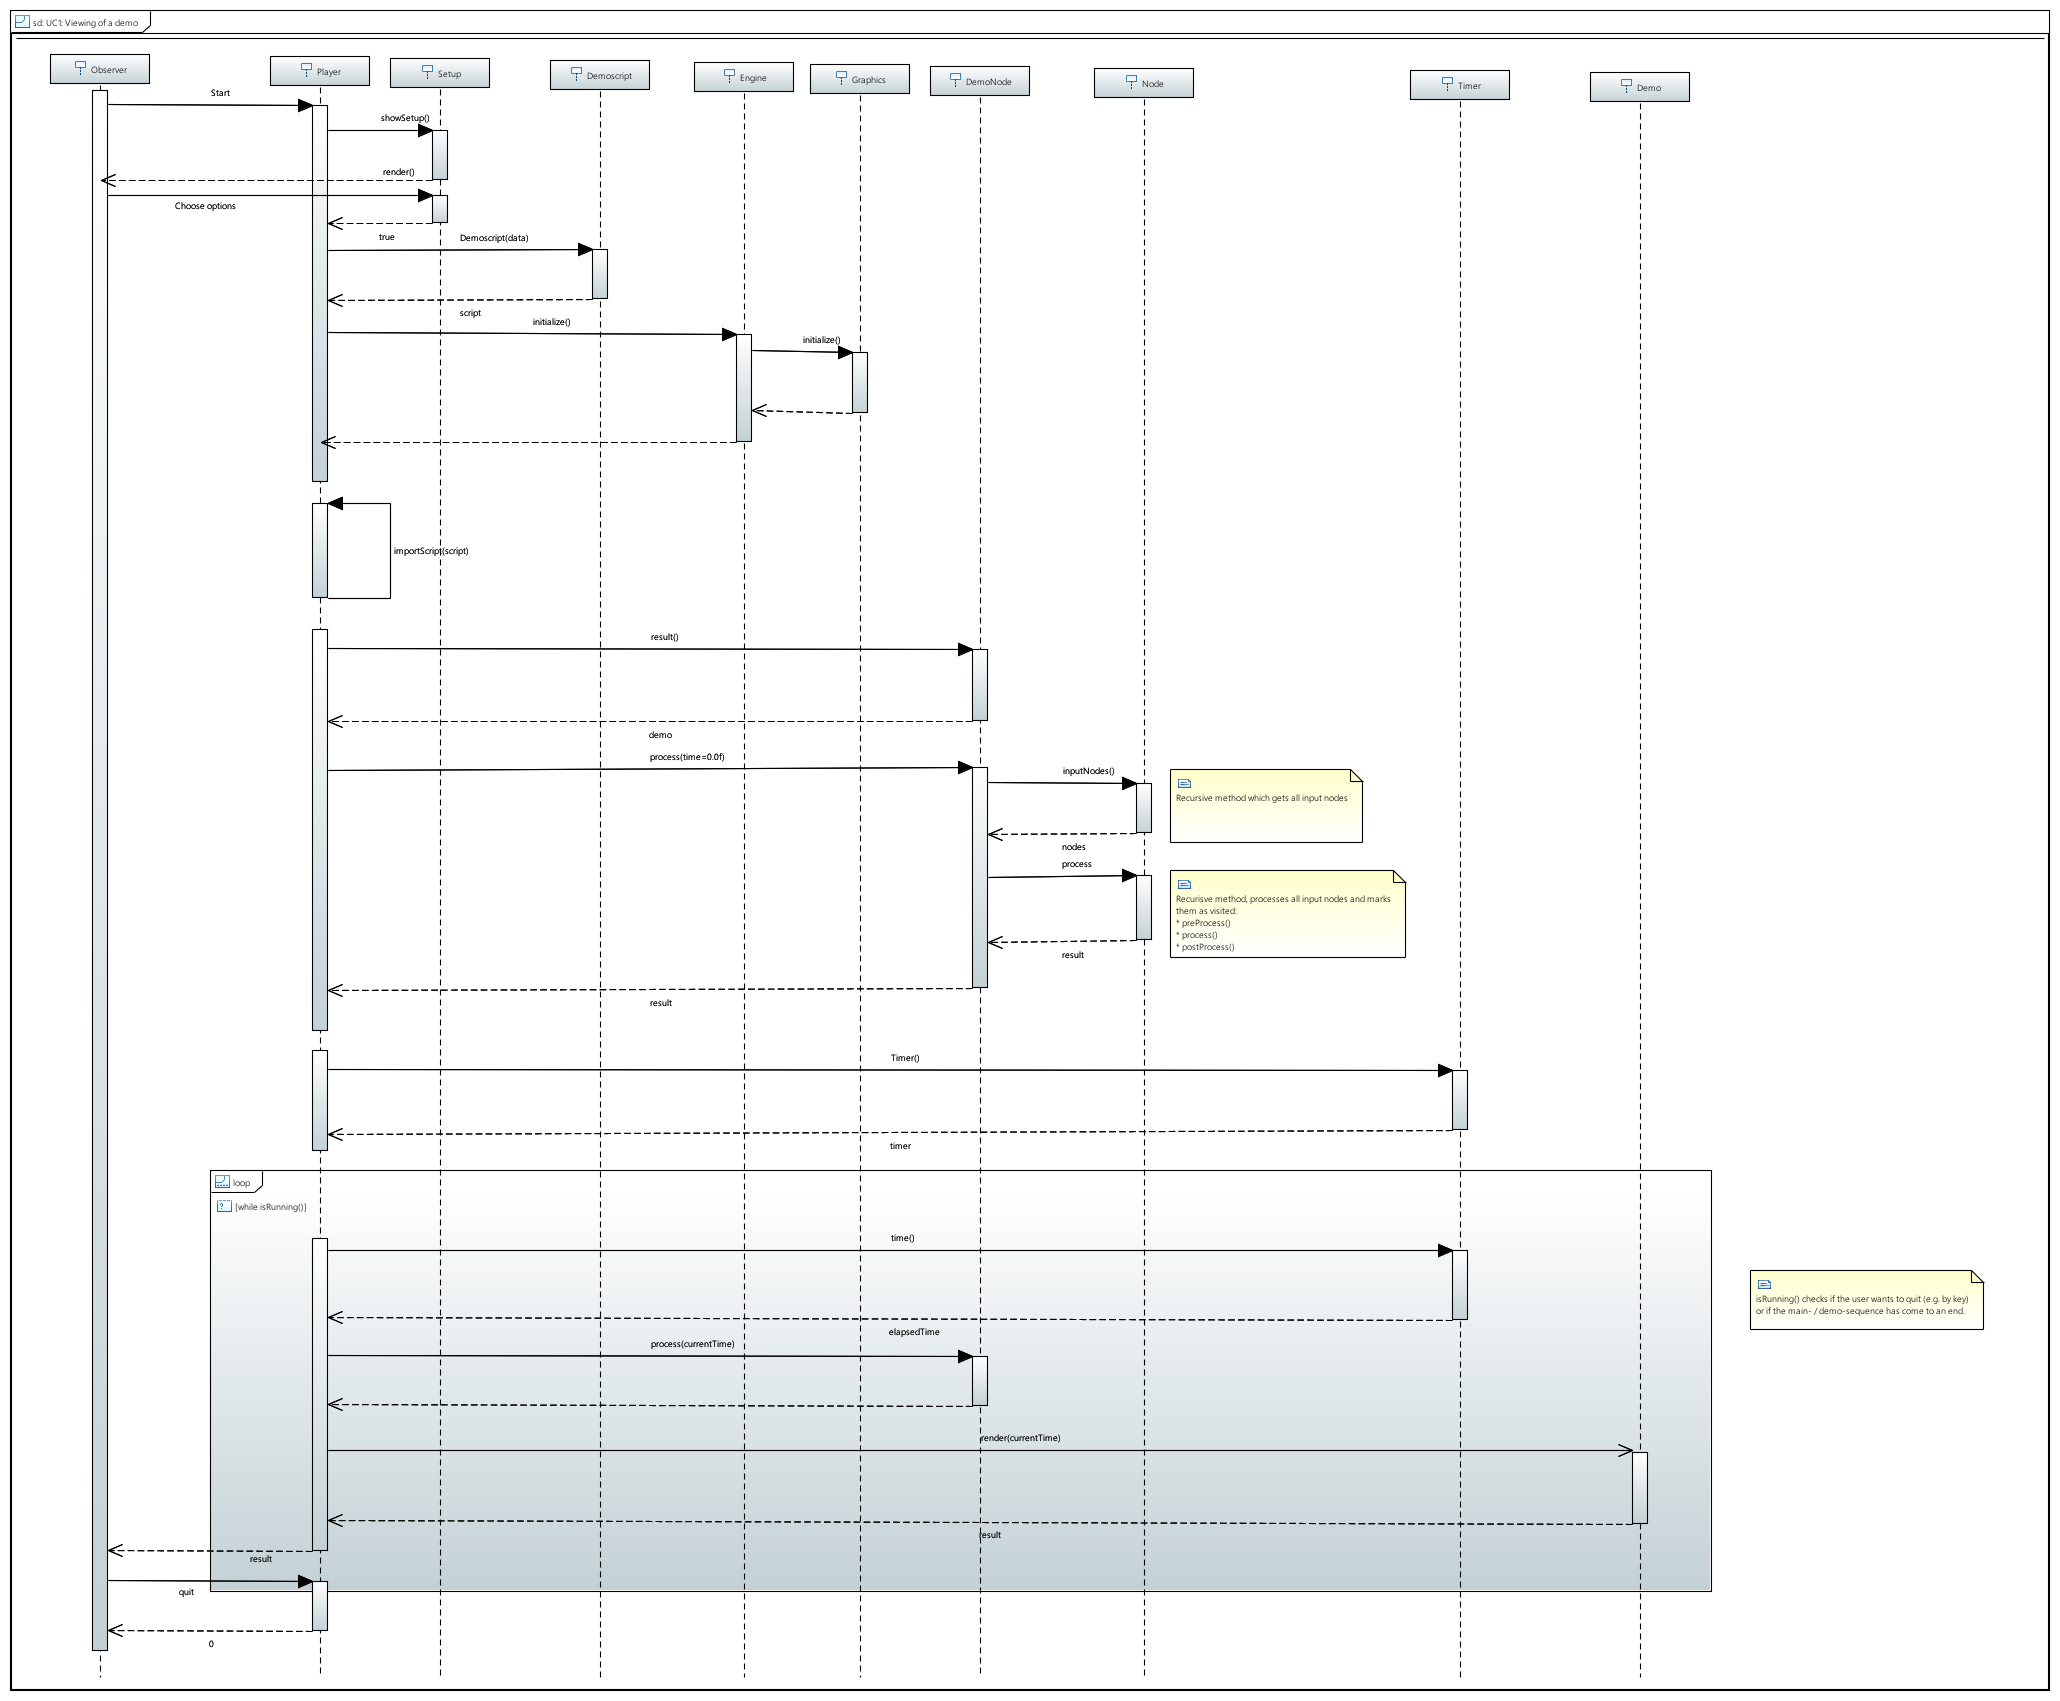
\includegraphics[angle=90,width=0.9\textwidth]{img/sequence_diagram_uc1.pdf}
    \caption{Sequenz-Diagramm  des Use Cases UC1
        \protect\footnotemark}\label{fig:package-diagram:editor}
\end{figure}
\footnotetext{Eigene Darstellung mittels Papyrus.}

\todo[inline]{Describe sequence diagram.}

% -*- coding: UTF-8 -*-
% vim: autoindent expandtab tabstop=4 sw=4 sts=4 filetype=tex
% vim: spelllang=de spell
% chktex-file 27 - disable warning about missing include files

\section{Logische Architektur}
\label{sec:logical-architecture}

Die logische Architektur zeigt das Gesamtbild der Software-Klassen in Form von
Paketen (bzw. Namespaces), Subsystemen und Layern~\cite{larman_applying_2004}.
Bei Layern handelt es sich um eine grobe Gruppierung von Klassen, Paketen oder
Subsystemen, welche zusammenhängen~\cite{larman_applying_2004}.

\subsection{Player}
\label{subsec:package-diagram:player}

\begin{figure}[H]
    \centering
    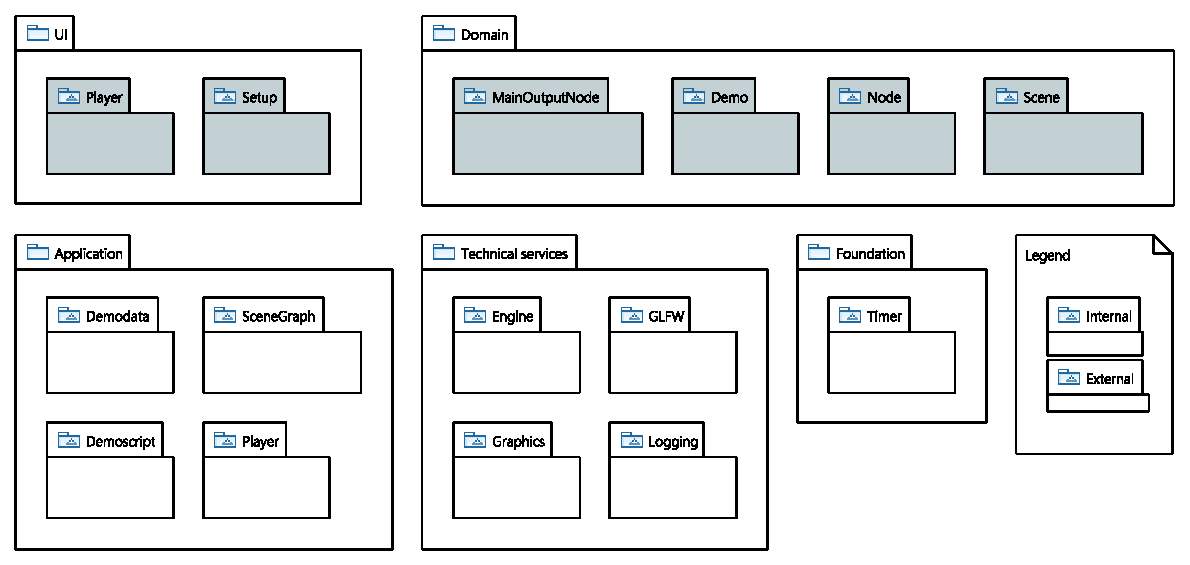
\includegraphics[width=0.7\textwidth]{img/player_package_diagram.pdf}
    \caption{Paket-Diagramm der
        Player-Applikation\protect\footnotemark}\label{fig:package-diagram:player}
\end{figure}
\footnotetext{Eigene Darstellung mittels Papyrus.}

\todo[inline]{Describe player package diagram.}

\subsection{Editor}
\label{subsec:package-diagram:editor}

\begin{figure}[H]
    \centering
    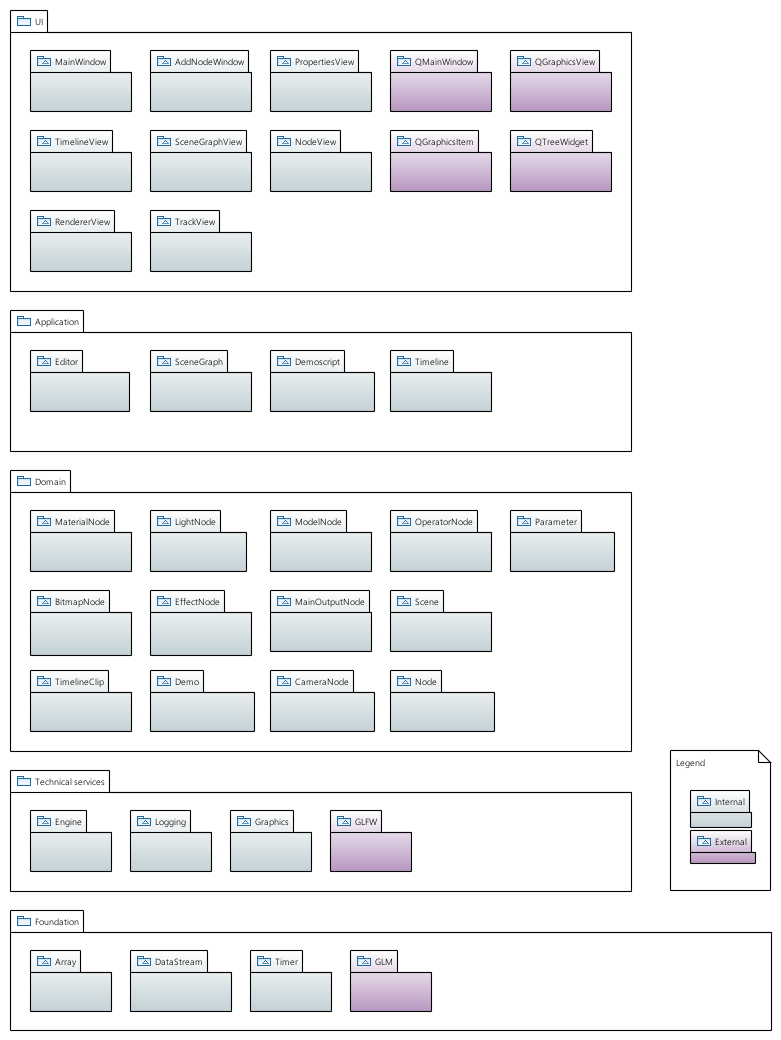
\includegraphics[width=0.9\textwidth]{img/editor_package_diagram.pdf}
    \caption{Paket-Diagramm der
        Editor-Applikation\protect\footnotemark}\label{fig:package-diagram:editor}
\end{figure}
\footnotetext{Eigene Darstellung mittels Papyrus.}

\todo[inline]{Describe editor package diagram.}

